% \documentclass[12pt]{article}
% % Options for packages loaded elsewhere
\usepackage{xcolor}
% In your preamble, open an output file:

\PassOptionsToPackage{unicode}{hyperref}
\PassOptionsToPackage{hyphens}{url}

% Basic packages
\usepackage{amsmath,amssymb}

% Remove section numbering
\setcounter{secnumdepth}{-\maxdimen}

% Font setup depending on engine
\usepackage{iftex}
\ifPDFTeX
  \usepackage[T1]{fontenc}
  \usepackage{textcomp} % provides euro and other symbols
\else % for LuaTeX or XeTeX
  \usepackage{unicode-math} % also loads fontspec
  \defaultfontfeatures{Scale=MatchLowercase}
  \defaultfontfeatures[\rmfamily]{Ligatures=TeX,Scale=1}
\fi

\usepackage{lmodern}

\usepackage[utf8]{inputenc}
\DeclareUnicodeCharacter{03B2}{\ensuremath{\beta}}
\DeclareUnicodeCharacter{1D6FD}{\ensuremath{\beta}}
\DeclareUnicodeCharacter{2248}{\ensuremath{\approx}}
\DeclareUnicodeCharacter{0394}{\ensuremath{\Delta}}
\DeclareUnicodeCharacter{0470}{\ensuremath{\Psi}}

% Use upquote if available (for straight quotes in verbatim)
\IfFileExists{upquote.sty}{\usepackage{upquote}}{}

% Use microtype if available
\IfFileExists{microtype.sty}{%
  \usepackage{microtype}%
  \UseMicrotypeSet[protrusion]{basicmath} % disable protrusion for tt fonts
}{}

% Adjust paragraph spacing for non-KOMA classes
\makeatletter
\@ifundefined{KOMAClassName}{%
  \IfFileExists{parskip.sty}{%
    \usepackage{parskip}%
  }{%
    \setlength{\parindent}{0pt}%
    \setlength{\parskip}{6pt plus 2pt minus 1pt}%
  }%
}{%
  \KOMAoptions{parskip=half}%
}
\makeatother

\usepackage{graphicx}

% Define a macro for scaling images to fit within the text area
\makeatletter
\newsavebox\pandoc@box
\newcommand*\pandocbounded[1]{%
  \sbox\pandoc@box{#1}%
  \Gscale@div\@tempa{\textheight}{\dimexpr\ht\pandoc@box+\dp\pandoc@box\relax}%
  \Gscale@div\@tempb{\linewidth}{\wd\pandoc@box}%
  \ifdim\@tempb\p@<\@tempa\p@\let\@tempa\@tempb\fi
  \ifdim\@tempa\p@<\p@\scalebox{\@tempa}{\usebox\pandoc@box}%
  \else\usebox{\pandoc@box}%
  \fi
}
\makeatother

% Set default figure placement to htbp
\def\fps@figure{htbp}

% Load color and highlighting packages for LuaTeX vs. others
% \ifLuaTeX
%   \usepackage{luacolor}
%   \usepackage[soul]{lua-ul}
% \else
%   \usepackage{soul}
% \fi

% Prevent overfull lines
\setlength{\emergencystretch}{3em}

% Define tight list formatting (from pandoc)
\providecommand{\tightlist}{%
  \setlength{\itemsep}{0pt}%
  \setlength{\parskip}{0pt}%
}

% Hyperlinks and bookmarks
\usepackage{bookmark}
\IfFileExists{xurl.sty}{\usepackage{xurl}}{} % allow URL line breaks
\urlstyle{same}
\hypersetup{
  hidelinks,
  pdfcreator={LaTeX via pandoc}
}

% Page geometry and additional formatting
\usepackage[margin=1in]{geometry}
\usepackage{lineno}   % for line numbering
\usepackage{setspace}

\usepackage[backend=biber, sorting=none,style=numeric-comp]{biblatex} % you can choose a different style if you like
%\usepackage[backend=biber]{biblatex} 
\addbibresource{references.bib} 

\usepackage{booktabs}  % For nicer horizontal lines
\usepackage{graphicx}

\usepackage{hyperref} % For clickable references and \phantomsection

% New counter for supplemental data
\newcounter{datafile}
\renewcommand{\thedatafile}{S\arabic{datafile}}

% Command for supplemental data sections
\newcommand{\datasection}[2]{%
  \refstepcounter{datafile}%
  \phantomsection%
  \noindent\textbf{Data \thedatafile.} #1%
  \label{#2}%
}

\usepackage{etoc}
\usepackage{lineno}

\usepackage{subcaption}
\renewcommand{\thesubfigure}{\Alph{subfigure}}
\captionsetup[subfigure]{
  labelformat=simple,
  labelsep=colon,
  justification=raggedright,
  singlelinecheck=off
}
\usepackage{subcaption}
\usepackage[normalem]{ulem}
\usepackage{longtable}
\usepackage{capt-of}

\usepackage[justification=raggedright, singlelinecheck=false]{caption}
\usepackage[belowskip=0pt]{caption}
\usepackage{float}
\usepackage{seqsplit}

% \begin{document}
\subsubsection*{Supplementary Figures}
\phantomsection
\addcontentsline{toc}{subsubsection}{Supplementary Figures}

\begin{figure}[H]
    \begin{subfigure}[t]{.2\textwidth}
        \caption{}
        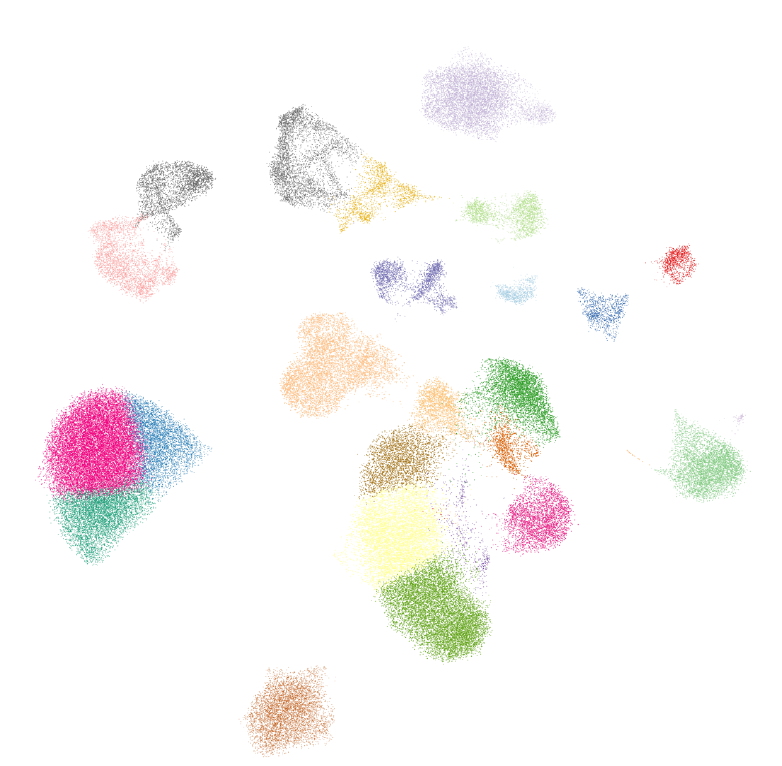
\includegraphics[width=\textwidth]{/Users/djuna/Documents/ABCA7lof2/editorial_paper/main_panels_svgs/fs1/cell_proj_with_leiden.pdf}        
    \end{subfigure}
    \begin{subfigure}[t]{.2\textwidth}
        \caption{}
        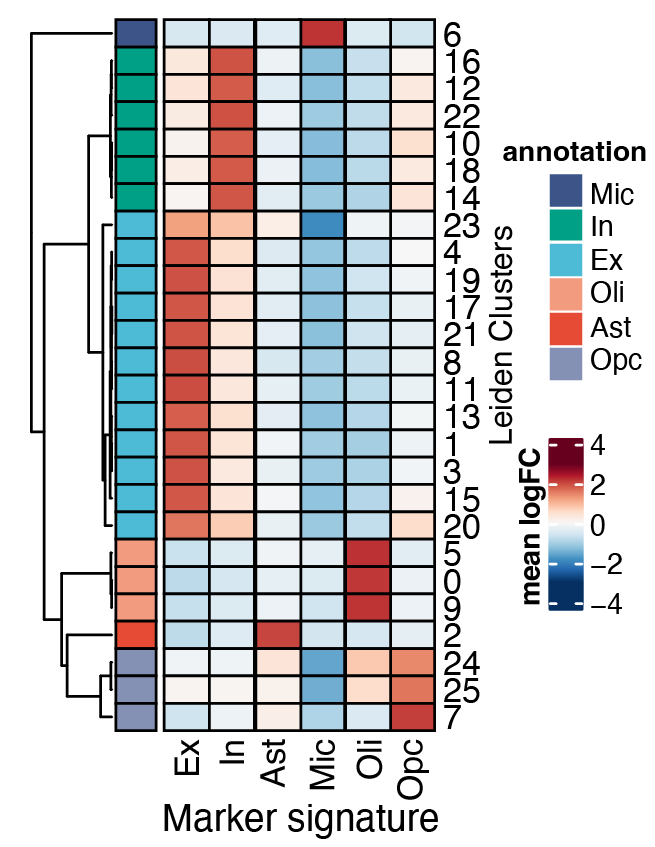
\includegraphics[width=\textwidth]{/Users/djuna/Documents/ABCA7lof2/editorial_paper/main_panels_svgs/fs1/leiden_heatmap.pdf}        
    \end{subfigure}   
    \begin{subfigure}[t]{.2\textwidth}
        \caption{}
        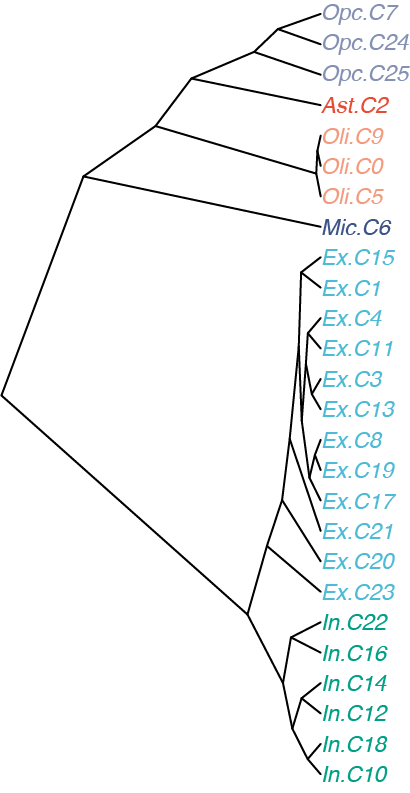
\includegraphics[width=\textwidth]{/Users/djuna/Documents/ABCA7lof2/editorial_paper/main_panels_svgs/fs1/hierarchical_tree.pdf}        
    \end{subfigure}  
    \begin{subfigure}[t]{.3\textwidth}
        \caption{}
        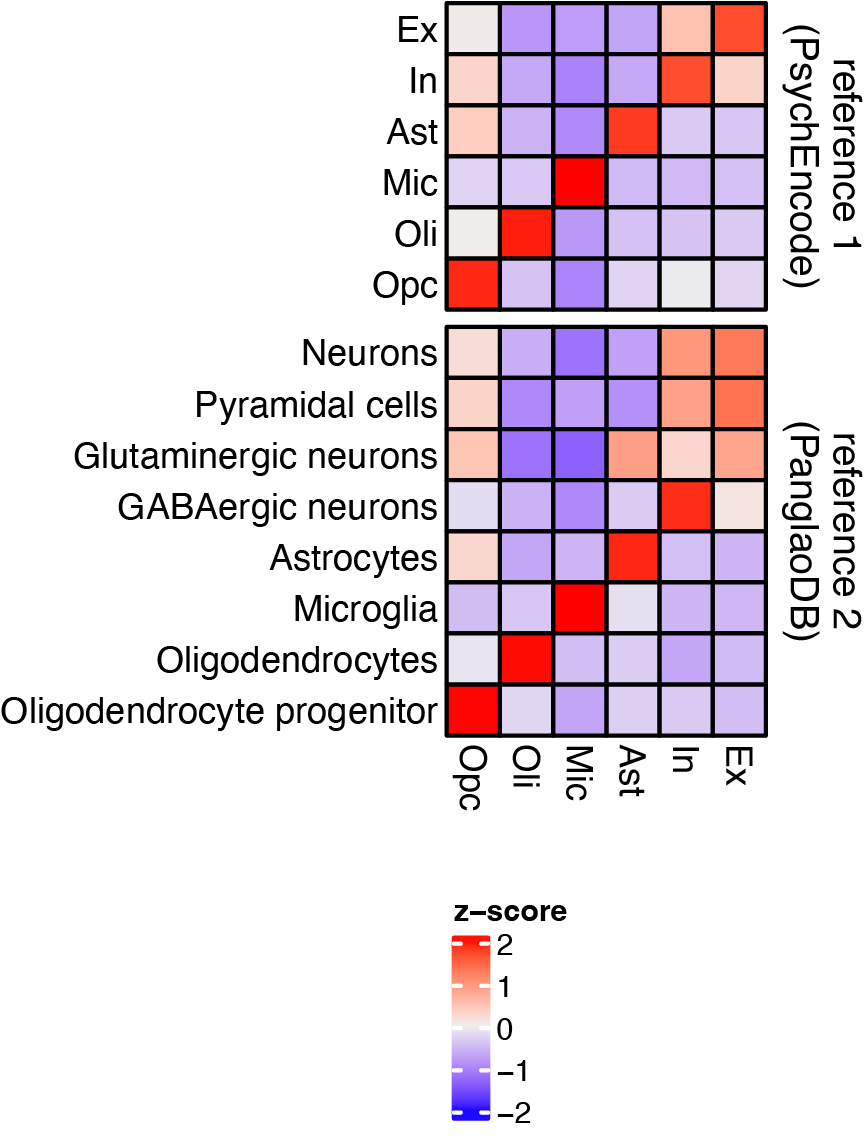
\includegraphics[width=\textwidth]{/Users/djuna/Documents/ABCA7lof2/editorial_paper/main_panels_svgs/fs1/marker_hmap.pdf}        
    \end{subfigure}  
    \begin{subfigure}[t]{.8\textwidth}
        \caption{}
        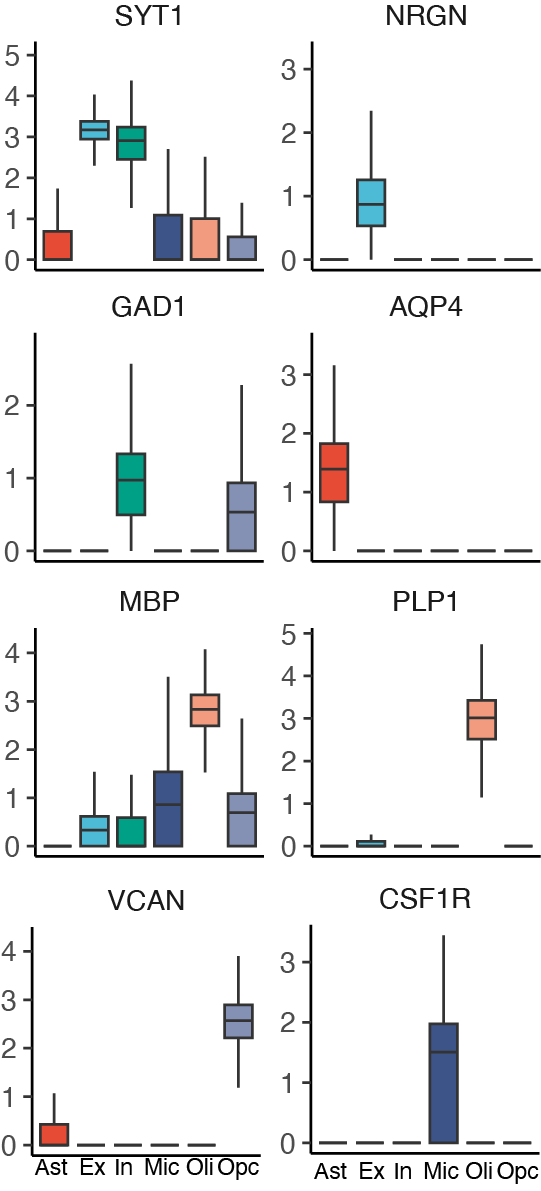
\includegraphics[width=\textwidth]{/Users/djuna/Documents/ABCA7lof2/editorial_paper/main_panels_svgs/fs1/marker_boxplot.pdf}        
    \end{subfigure}    
    \begin{subfigure}[t]{.2\textwidth}
        \caption{}
        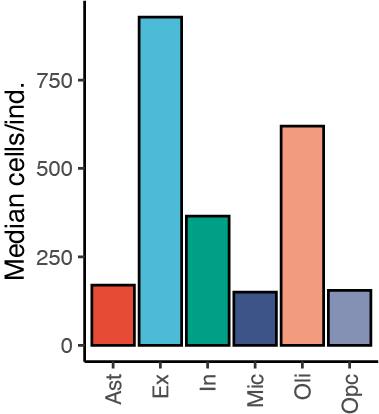
\includegraphics[width=\textwidth]{/Users/djuna/Documents/ABCA7lof2/editorial_paper/main_panels_svgs/fs1/median_cells.pdf}        
    \end{subfigure} 
    \begin{subfigure}[t]{.8\textwidth}
        \caption{}
        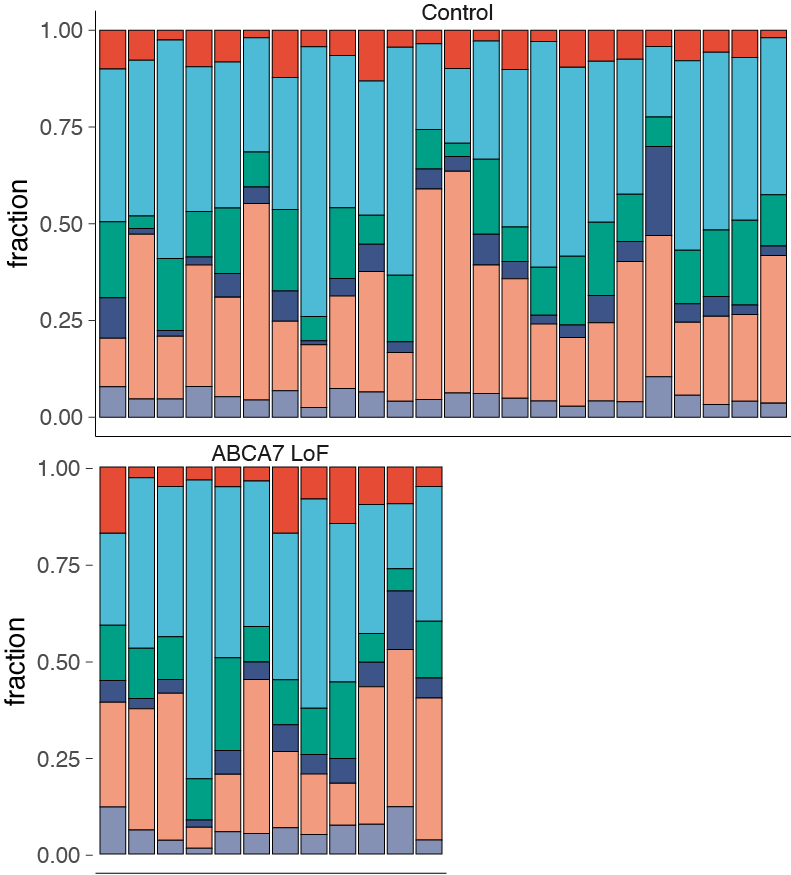
\includegraphics[width=\textwidth]{/Users/djuna/Documents/ABCA7lof2/editorial_paper/main_panels_svgs/fs1/individual_fractions.pdf}        
    \end{subfigure}  
    \begin{subfigure}[t]{.4\textwidth}
        \caption{}
        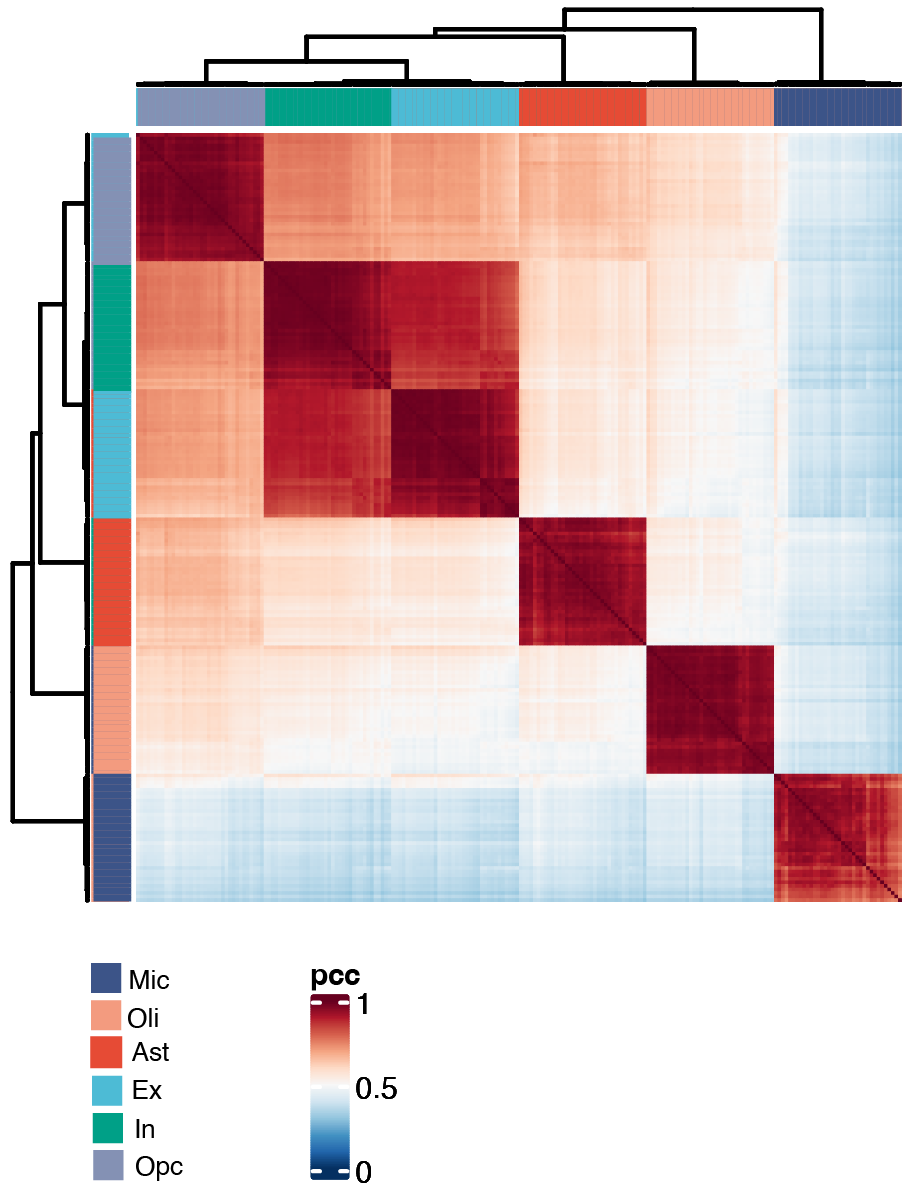
\includegraphics[width=\textwidth]{/Users/djuna/Documents/ABCA7lof2/editorial_paper/main_panels_svgs/fs1/celltype_heatmap.pdf}        
    \end{subfigure}  
    \begin{subfigure}[t]{.2\textwidth}
        \caption{}
        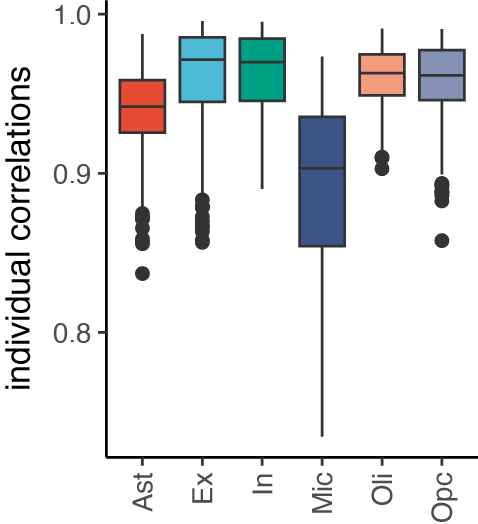
\includegraphics[width=\textwidth]{/Users/djuna/Documents/ABCA7lof2/editorial_paper/main_panels_svgs/fs1/individual_correlations.pdf}        
    \end{subfigure}
    \end{figure}


    \paragraph*{Fig. S2.} Overview of snRNA-sequencing cell type annotations.
    \phantomsection
    \addcontentsline{toc}{paragraph}{Fig. S1.}
    \textbf{a,} 2D UMAP projection of individual cells (N=102,710 cells, 32 subjects), colored by Leiden clusters.
    \textbf{b,} Average marker gene expression (mean log(fold-change) per cluster) for cell types (x-axis). Fold-changes calculated for each cluster versus all others, using marker genes from Reference 1 (Supplementary Table 3).
    \textbf{c,} Cladogram of subcluster relationships based on pairwise distances of per-cluster gene expression profiles.
    \textbf{d,} Average marker gene expression profiles per major cell type (y-axis) across two marker gene references (Supplementary Table 3).
    \textbf{e,} Per-cell distribution of selected marker gene expression by cell type (log-counts).
    \textbf{f,} Median number of cells per cell type per subject.
    \textbf{g,} Cell type fraction per subject.
    \textbf{h,} Heatmap showing correlations of individual-level gene expression profiles by cell type.
    \textbf{i,} Boxplots of individual-level gene expression correlations by cell type.
%\end{document}

